\newpage
%\null
%\cleardoublepage



%************************************************************************************************
% Kap5 Simulationsdurchfürhung
%************************************************************************************************

\chapter{Simulationsdurchführung}
\label{chap:Simulationsdurchfuehrung}

\section{Simulation}
In diesem Abschnitt werden verschiedene Simulationen durchgeführt.
Der Motor, der der Regelung zu Grunde liegt, ist der Gleichstrommotor aus der Vorlesung von Prof. Froriep.
Mit diesem Motor soll von einer Nullposition ausgehend ein Winkel von \unit[20]{°} angefahren werden. 
Dieser Winkel soll innerhalb von einer Millisekunde erreicht werden.

Es wird eine Spannungsbegrenzung von \unit[+/-24]{V} eingeführt, da diese eine in der Fertigung übliche Versorgungsspannung ist.

Zu Beginn wird der Sensor, der das aktuelle Positionssignal liefert, aus der Regelung heraus gelassen. 
Somit ist es möglich, die Regelung an den Motor anzupassen und sobald
diese die Sollwerte erfüllt, werden 3 verschiedene Sensoren das Positionssignal liefern.

\subsection{PID-Regelung}
\label{chap:pidregelung}
Für die verschiedenen P-, PI-, PD- und PID-Regelungen wird der PID-Reglerblock von Simulink verwendet.

Es wird mit einer P-Regelung begonnen, die Sollwerte zu erreichen. Wenn die P-Regelung nicht ausreicht, wird die P-Regelung erst nur um einen I-Anteil und dann nur um einen 
D-Anteil erweiteret. 
Sollten immernoch keine Zufriedenstellenden Ergebnisse vorliegen, so wird mit einer PID-Regelung versucht, die Vorgaben zu erreichen.

\subsubsection{P-Regelung}
\label{chap:p_regelung}
In Abb. \ref{fig:p40} ist das Ergebnis der reinen P-Regelung dargestellt. 
Es ist zu erkennen, dass nach ca. 7 ms es keine Veränderung des eingesetllten Winkels gibt. 
Eine Erhöhung des P-Anteils ergibt ein Überschwingen, wie es in Abb. \ref{fig:p45} dargestellt ist.
In Abb. \ref{fig:p40} und \ref{fig:p45} ist in der untersten Grafik der Sollwinkel sowie die angegebene Abweichung angezeigt. 
Wie zu erkennen ist, ist die verbleibende Regeldifferenz noch viel zu groß. 
Demnach wird mit einem zugefügten I-Anteil zur reinen P-Regelung versucht, die restliche große Regeldifferenz auszugleichen. 
Für die folgenden Simulationen wird das Matlab-File "msSpiegel_PID.m" und das Simulink-File "sSpiegel.slx" hergenommen.
\begin{figure}[!h]
	\centering
	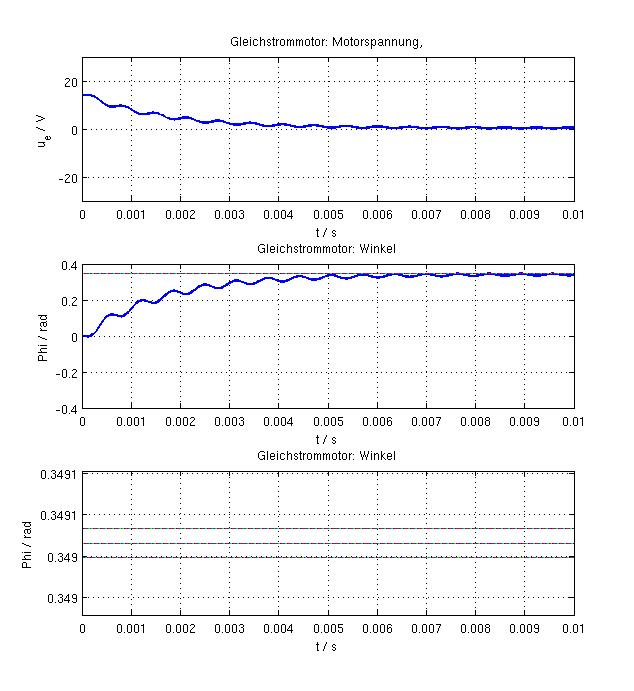
\includegraphics[width=0.6\textwidth]{NurP40.jpg}
	\caption{P-Anteil von 40}
	\label{fig:p40}
\end{figure}
\begin{figure}[!h]
	\centering
	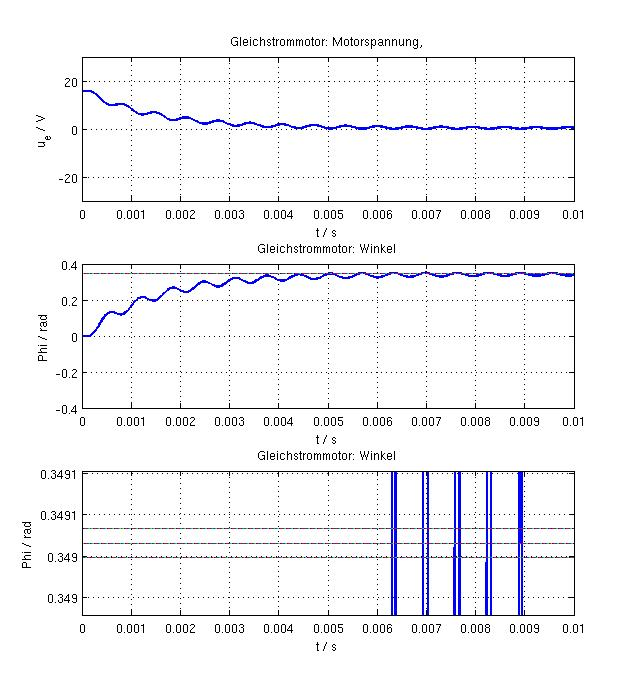
\includegraphics[width=0.6\textwidth]{NurP45.jpg}
	\caption{P-Anteil von 45}
	\label{fig:p45}
\end{figure}

\subsubsection{PI-Regelung}
\label{chap:pi_regelung}
In Abb. \ref{fig:p30i17} ist das Ergebnis der PI-Regelung dargestellt. 
Es ist zu erkennen, dass nach ca. 13 ms es keine Veränderung des eingesetllten Winkels gibt. 
Eine Erhöhung des P- oder I-Anteils ergibt ein Überschwingen, wie es in Abb. \ref{fig:p30i18} dargestellt ist.
In Abb. \ref{fig:p30i17} und \ref{fig:p30i18} ist in der untersten Grafik der Sollwinkel sowie die angegebene Abweichung angezeigt. 
Wie zu erkennen ist, ist die verbleibende Regeldifferenz noch viel zu groß. 
Demnach wird der zugefügte I-Anteil herausgenommen und ein D-Anteil zur reinen P-Regelung hinzugenommen, um so ein besseres Regelergebnis zu erreichen.
\begin{figure}[!h]
	\centering
	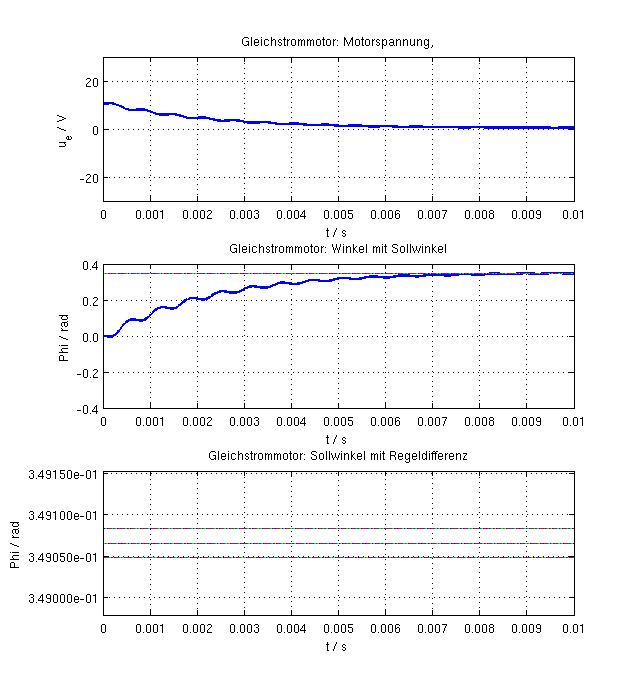
\includegraphics[width=0.6\textwidth]{PI-P30I17.jpg}
	\caption{P-Anteil von 30 und I-Anteil von 17}
	\label{fig:p30i17}
\end{figure}
\begin{figure}[!h]
	\centering
	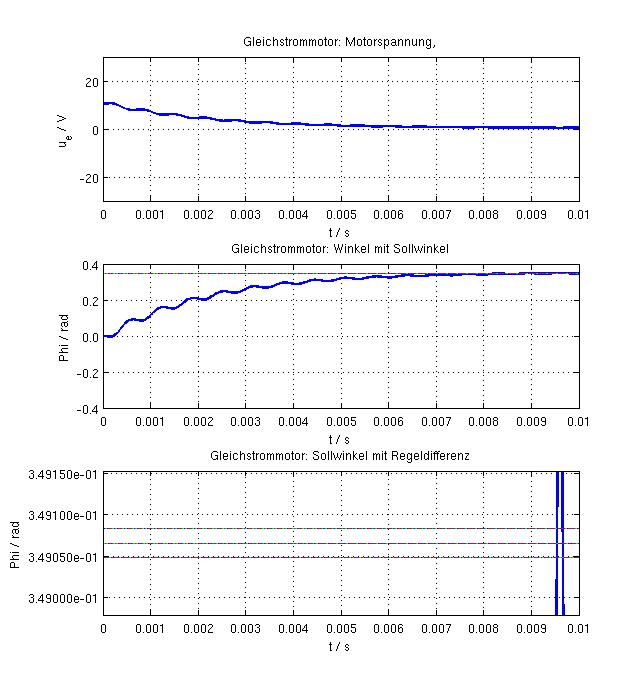
\includegraphics[width=0.6\textwidth]{PI-P30I18.jpg}
	\caption{P-Anteil von 30 und I-Anteil von 18}
	\label{fig:p30i18}
\end{figure}

\subsubsection{PD-Regelung}
\label{chap:pd_regelung}
Auch mit der PD-Regelung werden die Vorgaben noch nicht erfüllt. 
In Abb. \ref{fig:p22d1n1} ist das Ergebnis der PD-Regelung dargestellt. 
Es ist zu erkennen, dass nach ca. 7 ms es keine Veränderung des eingesetllten Winkels gibt. 
Eine Erhöhung des P- oder D-Anteils ergibt ein Überschwingen, wie es in Abb. \ref{fig:p23d1n1} dargestellt ist.
In Abb. \ref{fig:p22d1n1} und \ref{fig:p23d1n1} ist in der untersten Grafik der Sollwinkel sowie die angegebene Abweichung angezeigt. 
Wie zu erkennen ist, ist die verbleibende Regeldifferenz noch viel zu groß. 

\begin{figure}[!h]
	\centering
	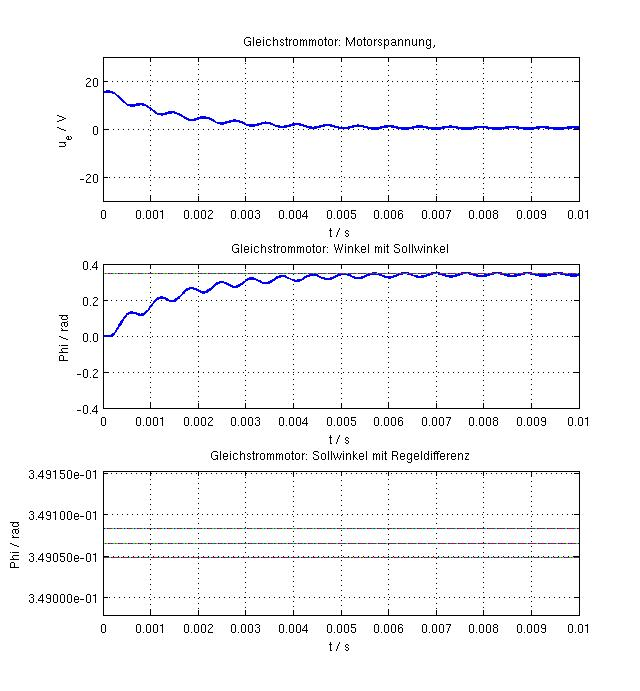
\includegraphics[width=0.6\textwidth]{PD-P22D1N1.jpg}
	\caption{P=22 - D=1 - N=1}
	\label{fig:p22d1n1}
\end{figure}
\begin{figure}[!h]
	\centering
	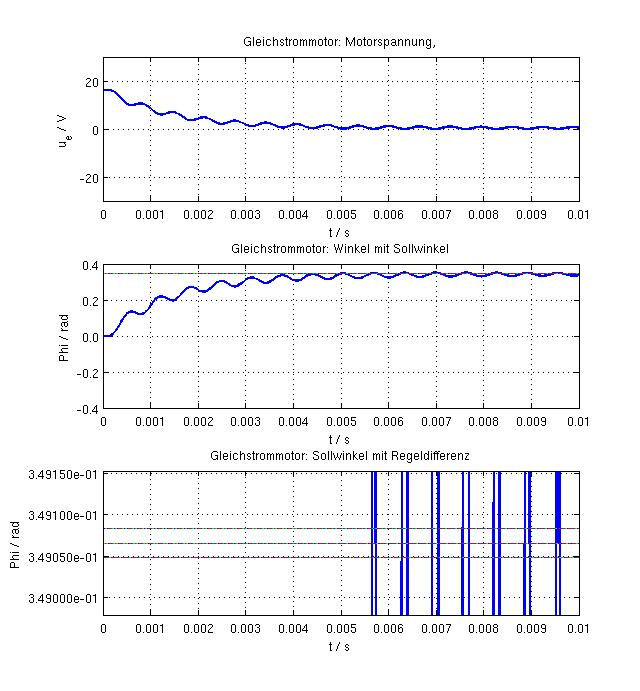
\includegraphics[width=0.6\textwidth]{PD-P23D1N1.jpg}
	\caption{P=22 - D=1 - N=1}
	\label{fig:p23d1n1}
\end{figure}
\subsubsection{PID-Regelung}
\label{chap:pid_regelung}
Nun wird mit einer Kombination der P-, I- und D-Anteile die Regelung betrieben.
In Abb. \ref{fig:p20i16d1n1} ist das Ergebnis der PID-Regelung dargestellt. 
Es ist zu erkennen, dass nach ca. 7 ms es keine Veränderung des eingesetllten Winkels gibt. 
Eine Erhöhung der verschiedenen Reglerparamteranteile ergibt ein Überschwingen, wie es in Abb. \ref{fig:p20i16d1n1} dargestellt ist.
In Abb. \ref{fig:p20i16d1n1} ist in der untersten Grafik der Sollwinkel sowie die angegebene Abweichung angezeigt.
Durch die große Abweichung vom Sollwinkel ist in dieser Grafik kein Graph zu erkennen.
\begin{figure}[!h]
	\centering
	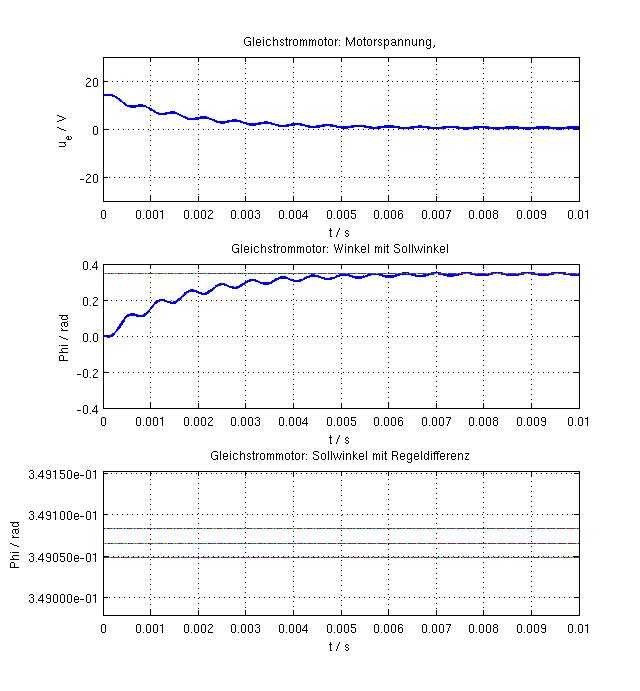
\includegraphics[width=0.6\textwidth]{PID-P20I15D1N1.jpg}
	\caption{P=20 - I=15 - D=1 - N=1}
	\label{fig:p20i15d1n1}
\end{figure}
\begin{figure}[!h]
	\centering
	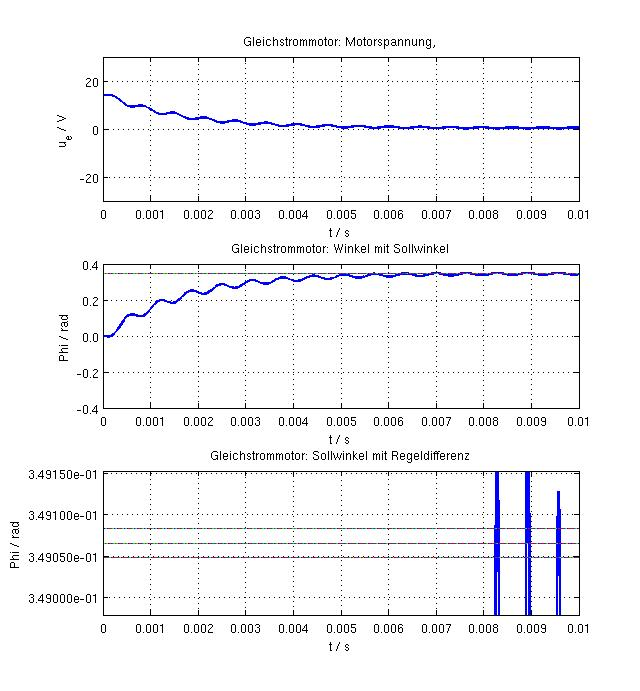
\includegraphics[width=0.6\textwidth]{PID-P20I16D1N1.jpg}
	\caption{P=20 - I=16 - D=1 - N=1}
	\label{fig:p2oi16d1n1}
\end{figure}

\subsection{P-Adaption}
\label{chap:padaption}
Es zeigt sich, dass der P-Anteil den meisten Einfluss, bzw. den größten Erfolg bei der Regelung ausmacht. 
Durch hinzugefügte I- oder D-Anteile konnte die Regelung nicht verbessert werden.
Nach dem die verschiedenen Regler die Vorgaben noch nicht erfüllen konnten, wird nun die P-Adapion eingesetzt. 
Bei der P-Adaption wird folgende Formel vor den P-Verstärker geschaltet:
\begin{center}
\begin{equation}
f = 1 + \frac {c_1 - 1}{(c_2 * e)^2 + 1}
\end{equation}
\end{center}
Dabei muss der Regelkreis folgendermaßen erweitert werden:
\begin{figure}[!h]
	\centering
	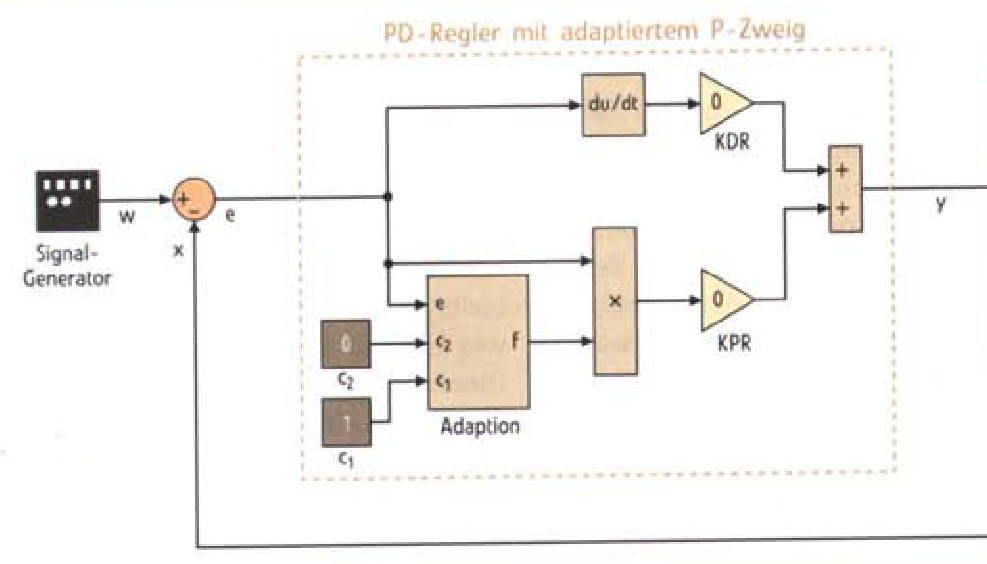
\includegraphics[width=0.6\textwidth]{P-Adaption.jpg}
	\caption{P-Adaption\cite{FrKu}}
	\label{fig:padaption}
\end{figure}
FrKu: PDF, "Tempo beim Laserzugriff", Artikel im F&M Elektronik, Jahrg.111(2003)5, Lugmair, Froriep, Kuplent, Langhans
Eine Integration in das bestehende Simulinkprogramm ist in Abb. \ref{} dargestellt.
\begin{figure}[!h]
	\centering
	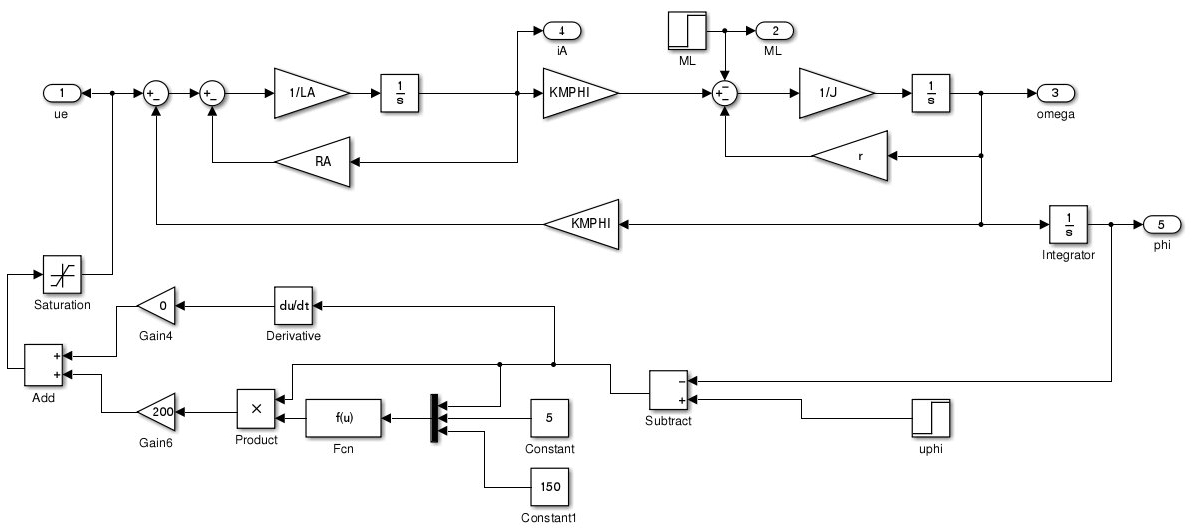
\includegraphics[width=0.6\textwidth]{sSpiegelPad.jpg}
	\caption{P-Adaption in Simulink
	\label{fig:padaptionsimulink}
\end{figure}

\subsubsection{Regelung mit P-Adaption}
\label{chap:p_adaption}
Nun kann mit drei verschiedenenn Parametern verucht werden, die Sollwerte zu erreichen.
Wobei die beiden f-Parameter zu Beginn auf 1 gesetzt werden und erst mit dem erhöhen des P-Anteils versucht wird, eine gute Regelung zu erhalten. 
Danach werden die beiden f-Parameter einzeln erhöht bzw. erniedrigt, bis sich das Erebniss verbessert hat. 
Eine Anpassung des P-Anteils und danach eine erneute Anpassung der f-Parameter gehört ebenso zur Erreichung einer passenden Regelung.
Für die folgenden Simulationen wird das Matlab-File "msSpiegel_Pad.m" und das Simulink-File "sSpiegelPad.slx" hergenommen.
\begin{figure}[!h]
	\centering
	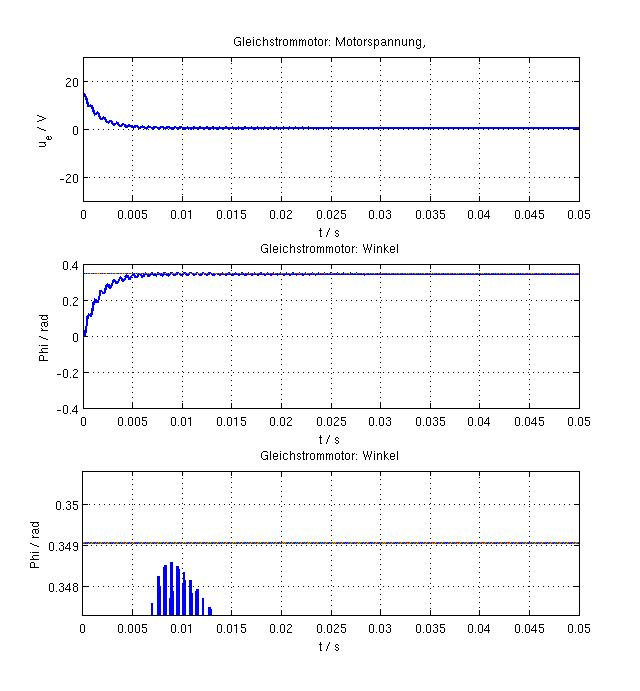
\includegraphics[width=0.6\textwidth]{Pad-P41F1_1,5F2_80.jpg}
	\caption{P-Adaption mit Parametern}
	\label{fig:padp41f1580}
\end{figure}
In Abb. \ref{fig:padp41f1580} ist zu erkennen, dass der Sollwinkel nicht erreicht wird. 
Wird jedoch der P-Anteil erhöht und mit den beiden f-Parametern weitere Einstellungen probiert, so wird der Sollwinkel nie erreicht. 
Es kommt zwar zu einem Schwingen um den Sollwinkel, aber dieser kann nicht stabil erreicht werden, siehe Abb. \ref{fig:padp50f3400}.
\begin{figure}[!h]
	\centering
	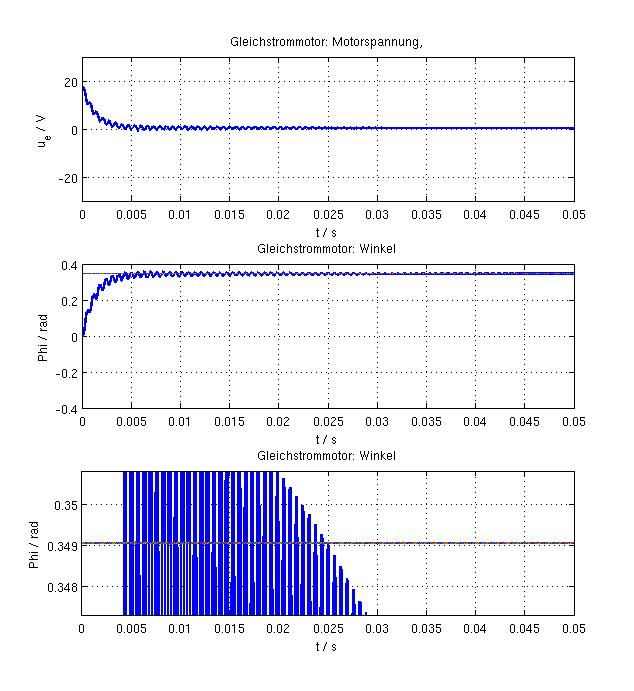
\includegraphics[width=0.6\textwidth]{Pad-P50F1_3F2_400.jpg}
	\caption{P-Adaption mit Parametern}
	\label{fig:padp50f3400}
\end{figure}

\subsubsection{P-Adaption mit Galvo-Werten}
\label{chap:p_adaptiongalvo}
Durch die Verwendung der P-Adaption konnte die Einregelzeit nicht verbessert werden.
Es zeigt sich, dass mit dem vorhandenen Gleichstrommoter keine der Vorgaben eingehalten werden können.
Um heraus zu finden, welche Daten der Motor aufweisen müsste, um mit einer PID- oder P-Adaption geregelt werden zu könnnen, werden jetzt zusätzlich zu den $f_{1}$ und $f_{2}$
Parametern auch die Motorparameter geändert.
Beispielhaft wurden Werte für den Innenwiderstand und der Induktivität eines Galvos 6230 der Firma Cambridge Technology als Grundlage verwendet \cite{CaTe}.

CaTe: PDF, Model 6230H Optical Scanner (Mechanical and Electrical Specifications), Cambridge Technology, 03/07.

Für die folgenden Simulationen wird das Matlab-File "msSpiegel_Pad_Werte.m" und das Simulink-File "sSpiegelPad.slx" hergenommen.

In Abb. \ref{fig:padwerte} ist eine langsame Annäherung an die zu erfüllenden Vorgaben zu sehen. 
Jedoch noch nicht in der geforderten Zeit und noch mit zu großen Schwankungen um den Sollwinkel.
Es sind folgende Werte aktuell eingestellt:
\begin{itemize}
\item Innenwiderstand der Spule: 1.07 \Omega
\item Induktivität der Spule: 173 \mu H
\item P-Anteil: 330
\item $f_1$: 5
\item $f_2$: 370
\end{itemize
}
\begin{figure}[!h]
	\centering
	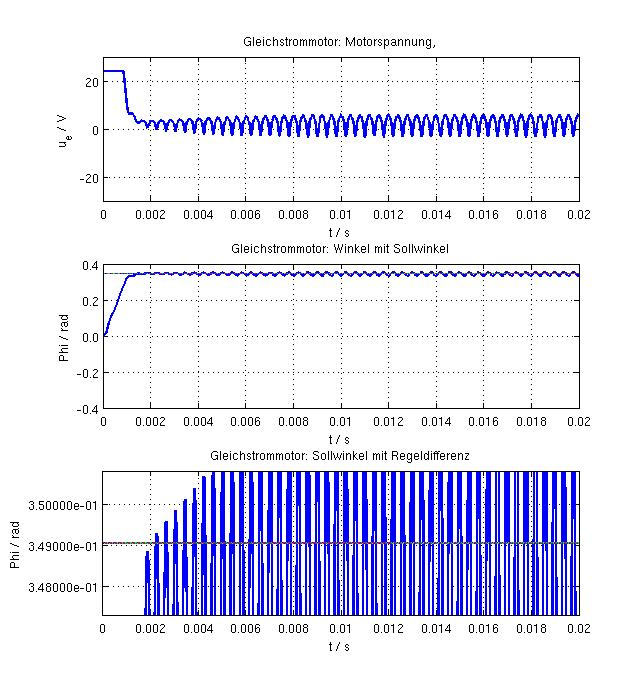
\includegraphics[width=0.6\textwidth]{Pad-Werte-P330F1_5F2_370.jpg}
	\caption{P-Adaption mit neuen Motorparametern}
	\label{fig:padwerte}
\end{figure}

\subsubsection{P-Adaption mit neuen Werten}
\label{chap:p_adaptionwerte}
Nun werden die Motor- und Spiegelwerte solange verändert, bis sich das gewünschte Ergebniss einstellt. 
Sollte die Regelung erfolgreich sein, könnte mit den veränderten Werten evtl. ein Motor und Spiegel hergestellt werden, der den Anforderungen entspricht.

Für die folgenden Simulationen wird das Matlab-File "msSpiegel_Pad_Neue_Werte.m" und das Simulink-File "sSpiegelPad.slx" hergenommen.
\begin{figure}[!h]
	\centering
	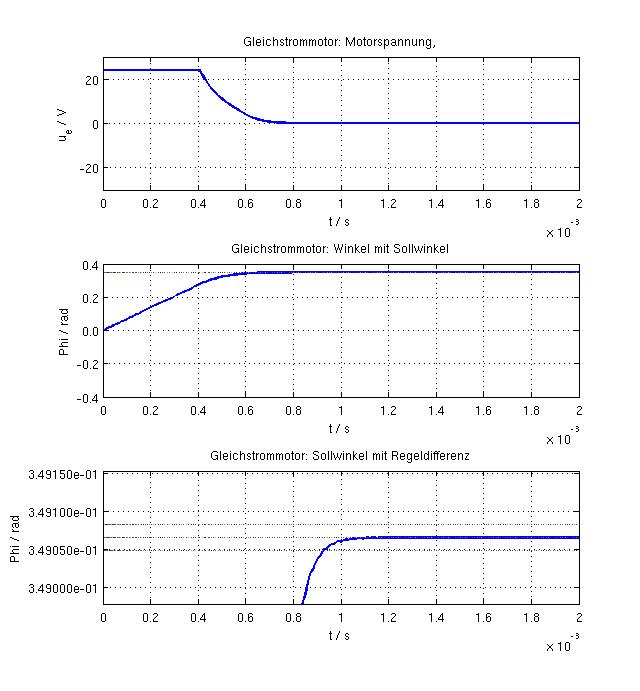
\includegraphics[width=0.6\textwidth]{Pad-Neue-Werte-P320F1_2F2_65.jpg}
	\caption{P-Adaption mit neuen Parametern}
	\label{fig:padneuewerte}
\end{figure}
Wie in Abb. \ref{fig:padneuewerte} zu erkennen, ist die Regelung in den geforderten Bereichen erfolgreich.
Der geforderte Winkel von 20{\textdegree} ist unter 1ms in seinen Regeldifferenzen erreicht. 
Dieser Regelung liegen folgende Werte zu Grunde:
\begin{itemize}
\item Innenwiderstand der Spule: 0.1 \Omega
\item Induktivität der Spule: 3 \mu H
\item Motorkonstante KMPHI: 35e-3 Vs
\item Reibungskoeffizient: 6e-5 Nm*s
\item Trägheitsmoment des Spiegels: 93.3e-9 $kg*m^2$
\item Drehmoment auf den Spiegel:130.25e-6 Nm
\item P-Anteil: 320
\item $f_1$: 2
\item $f_2$: 160
\end{itemize}

\subsubsection{Strombegrenzung}
\label{chap:p_adaptionstrom}
Ein Blick auf den Strom liefert allerdings Ergebnisse, die weiterer Überarbeitung der Regelung bedürfen.
In Abb. \ref{fig:stromzuhoch} ist der Strom der aktuellen Regelung dargestellt. 
Es fliessen Ströme in Höhe von 80 A.
\begin{figure}[!h]
	\centering
	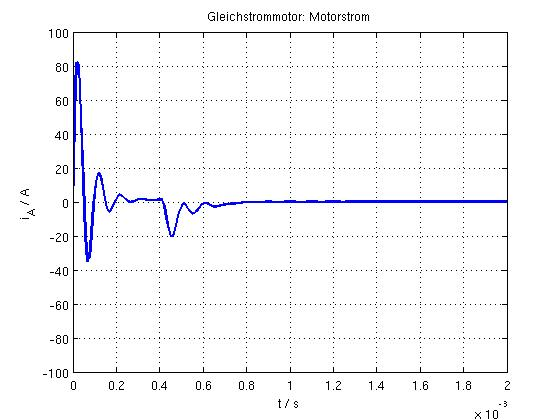
\includegraphics[width=0.6\textwidth]{Strom_zu_hoch.jpg}
	\caption{Stromhöhe während der Regelung}
	\label{fig:stromzuhoch}
\end{figure}
Dies ist allerdings sehr hoch, deshalb wird in die bestehende Regelung eine Strombegrenung von 10 A eingebaut und erneut versucht, die Regelung entsprechende anzupassen.
\begin{figure}[!h]
	\centering
	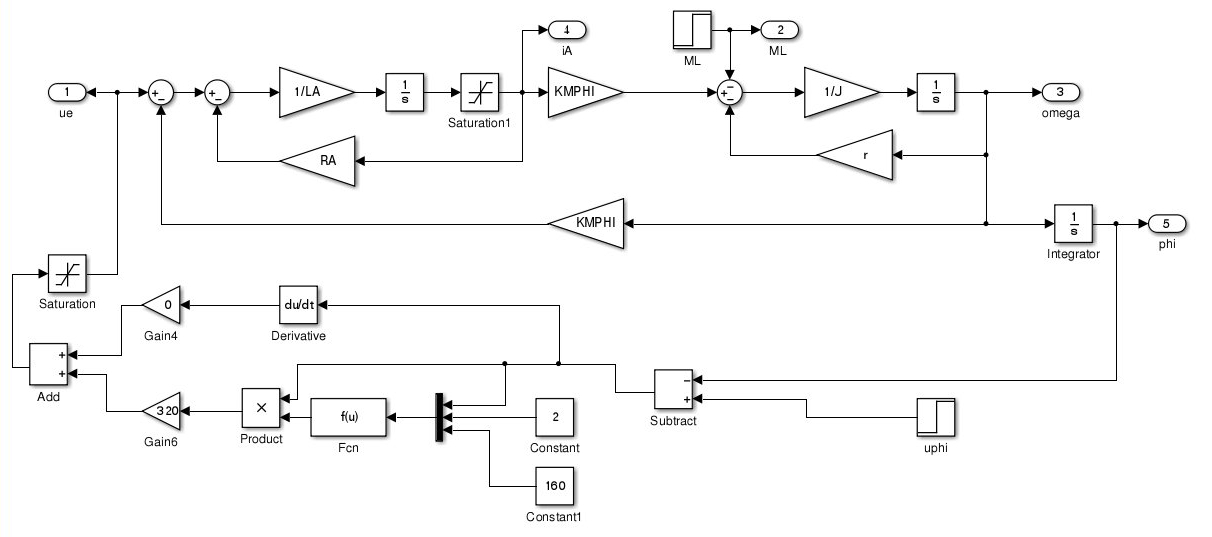
\includegraphics[width=0.6\textwidth]{P-Adaption-Strom.jpg}
	\caption{P-Adaption mit Strombegrenzung}
	\label{fig:strombegrenzt}
\end{figure}
In Abb. \ref{fig:strombegrenzt} ist die P-Adaption mit einer Strombegrenzung zu erkennen. 
Für eine bessere Übersicht, wurden entsprechende Positionen mit einem Namen versehen und der D-Anteil aus der Regelung genommen, da dieser auf Null gesetzt ist, siehe
Abb. \ref{fig:strombegrenztsauber}.
\begin{figure}[!h]
	\centering
	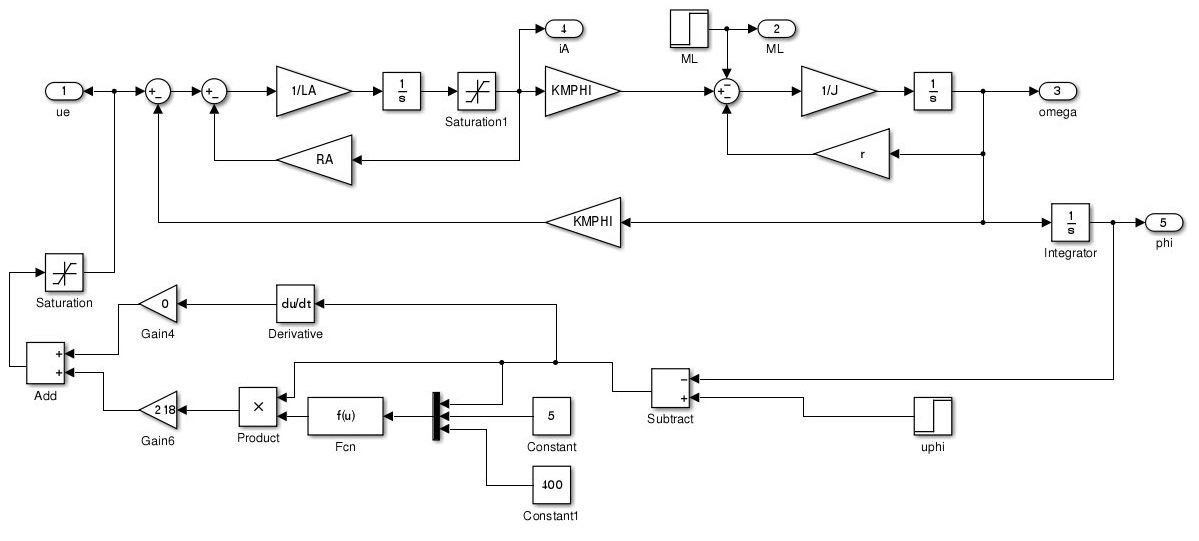
\includegraphics[width=0.6\textwidth]{sSpiegelPadStrom.jpg}
	\caption{Stromhöhe während der Regelung}
	\label{fig:strombegrenztsauber}
\end{figure}
Für die folgenden Simulationen wird das Matlab-File "msSpiegel_Pad_Neue_Werte_Strom.m" und das Simulink-File "sSpiegelPadStrom.slx" hergenommen.

Eine Regelung mit den aktuellen Werten zeigt das in Abb. \ref{fig:strombegrenztpad} zu erkennende Ergebnis.
\begin{figure}[!h]
	\centering
	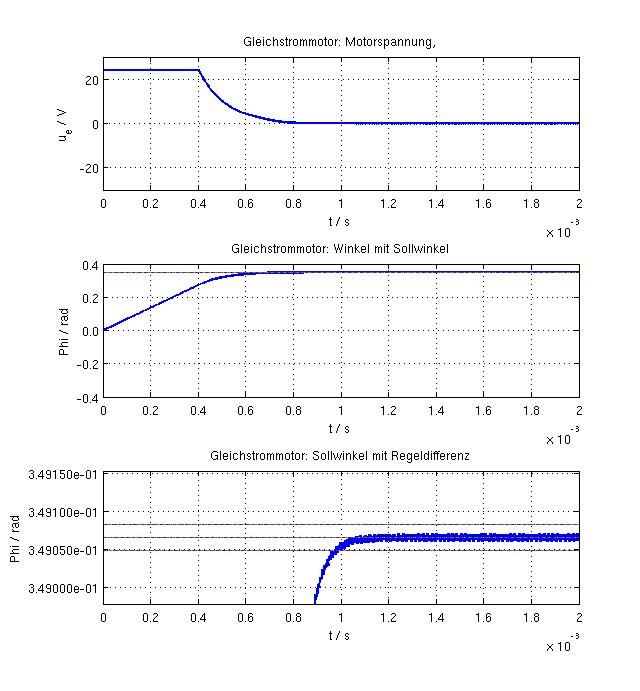
\includegraphics[width=0.6\textwidth]{Strom-Pad-Neue-Werte-P320F1_2F2_160.jpg}
	\caption{P-Adaption mit Strombegrenzung}
	\label{fig:strombegrenztpad}
\end{figure}
Durch weiteres Anpassen der unterschiedlichen Parameter, konnten die Sollwerte fast erreicht werden. 
Abb. \ref{fig:strombegrenztpadfastsoll} zeigt schon ein sehr gutes Ergebnis.
\begin{itemize}
\item Neues Trägheitsmoment des Spiegels: 93.3e-11 $kg*m^2$
\item Neues Drehmoment auf den Spiegel: 30,25e-6 Nm
\item P-Anteil: 218
\item $f_1$: 5
\item $f_2$: 400
\end{itemize}
\begin{figure}[!h]
	\centering
	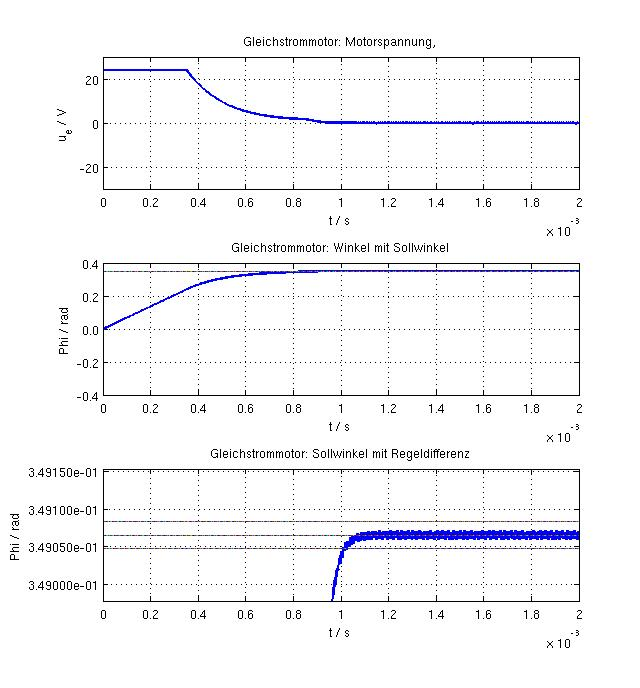
\includegraphics[width=0.6\textwidth]{Strom-Pad-Neue-Werte-P218F1_5F2_400.jpg}
	\caption{Angepasste P-Adaption mit Strombegrenzung}
	\label{fig:strombegrenztpadfastsoll}
\end{figure}

\subsubsection{Fertige P-Adaption}
\label{chap:p_adaptionfertig}
Die Einregelzeit liegt nur noch knapp über der vorgegebenen Zeit, durch weitere Anpassung der Regelparameter soll die vorgegebene Einregelzeit erreicht werden.
Abb. \ref{}
\begin{figure}[!h]
	\centering
	\includegraphics[width=0.6\textwidth]{Strom-Pad-Neue-Werte-P250F1_3F2_160.jpg}
	\caption{Angepasste P-Adaption mit Strombegrenzung}
	\label{fig:strombegrenztpadsoll}
\end{figure}
\begin{itemize}
\item Trägheitsmoment des Spiegels: 93.3e-11 $kg*m^2$
\item Drehmoment auf den Spiegel: 30,25e-6 Nm
\itemP-Anteil: 250
\item $f_1$: 3
\item $f_2$: 150
\end{itemize}
In Abb. \ref{fig:strombegrenztpadsoll} ist zu erkennen, dass durch Anpassung des Trägheitsmoments des Spiegels, des wirkenden Drehmoments auf den Spiegel und der verschiedenen
Regelparameter, trotz Spannungs- und Strombegrenzung, die Regelung erfolgreich ist. 
Der Spiegel zittert zwar etwas um die Position, dies ist aber im angegebenen 
Toleranzbereich.

\subsection{Regelung mit Sensor}
\label{chap:sensorregelung}
Nach dem die Regelung für einen perfekt linear arbeitenden Sensor, der durch ein direktes abgreifen des aktuellen Winkels realisiert wurde, funktioniert, wird der Sensor 
aus Kap \ref{chap:sensor} in die Simulation mit eingebaut.
Dafür wird das vorhandene Simulink-File "sSpiegelPadStrom.slx" hergenommen und um den Sensor erweitert.
Zudem wird der eingegebene Winkel in eine Spannung umgerechnet, da der Sensor eine vom Winkel abhängige Spannung ausgibt.
In Abb. \ref{fig:simusensor} ist der gesamte Simulationsaufbau dargestellt, welcher als "sSpiegelPadStromSensor.slx" gespeichert ist.
\begin{figure}[!h]
	\centering
	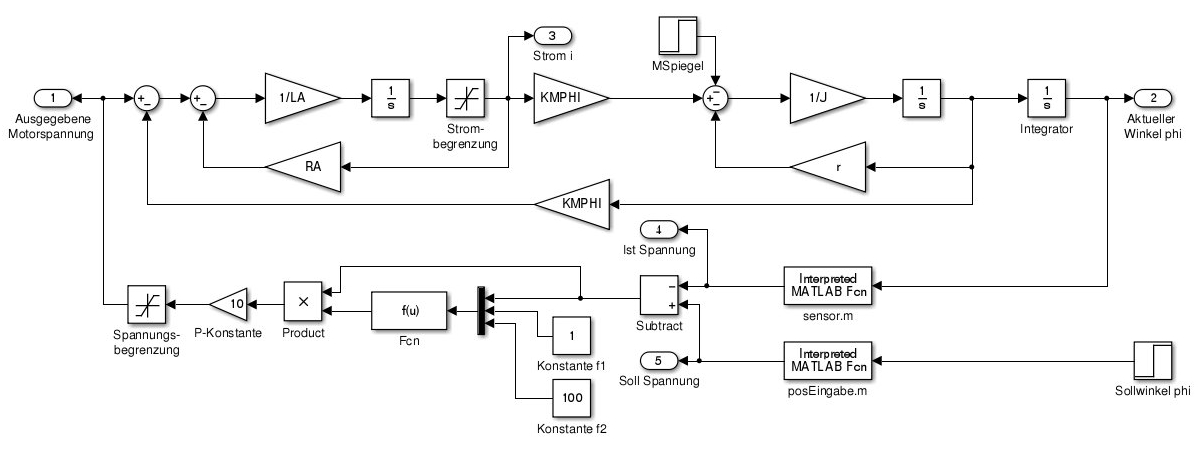
\includegraphics[width=0.6\textwidth]{sSpiegelPadStromSensor.jpg}
	\caption{Simulinaufbau mit Sensor}
	\label{fig:simusensor}
\end{figure}
Zur Ansteuerung wird das Matlab-File "msSpiegel_Pad_Neue_Werte_Strom.m" modifiziert und als "msSpiegelundSensor.m" gespeichert.
In diesem Matlab-File ist es möglich, verschiedene Kenndaten für den Sensor einzugeben.
Es werden folgende Daten hergenommen:
\begin{itemize}
\item Innenradius = 5 mm
\item Aussenradius = 10 mm
\item Lastwiederstand = 6000 Ohm
\item Messbereich = 20/180*pi (20°)
\item LEDLeistung = 1 W
\item Umgebungstemperatur = 300 K
\item nonlinear = 0.0001 (falls ein nichtlinearer Sensor simuliert werden soll)
\end{itemize}

Es werden drei verschieden Simulationen durchgeführt.

In der ersten Simulation wird ein linearen Sensor verwendet.
Dies sollte die gleichen Ergebnisse liefern wie der ideale Sensor.
Hierbei wird die Regelung, falls nötig, angepasst.

Die zweite Simulation wird ebenfalls mit einem linearen Sensor durchgeführt, nur ist hierbei die Linearität durch eine Faltung der Blende mit der Sensorfläche realisiert 
worden.
Es wird erwartet, dass sich dieser Sensor gleich verhält wie der ideale Sensor.

Bei der dritten und letzten Simulation wird ein nichtlinearer Sensor verwendet. 
Wobei der Nichtlinearitätsfaktor, der Werte zwischen 0 und 1 annehmen kann, auf den Wert 0,0001 gesetzt wird.
Dies sollte ein nahezu lineares Verhalten zeigen.

\subsubsection{Linearer Sensor 1}
\label{chap:sensorregelung1}
Abb. \ref{fig:linear1} zeigt das Regelergebnis des ersten linearen Sensors.
Es ist gut zu erkennen, dass die Regelung sogar schneller Erfolgt als vorher.
\begin{figure}[!h]
	\centering
	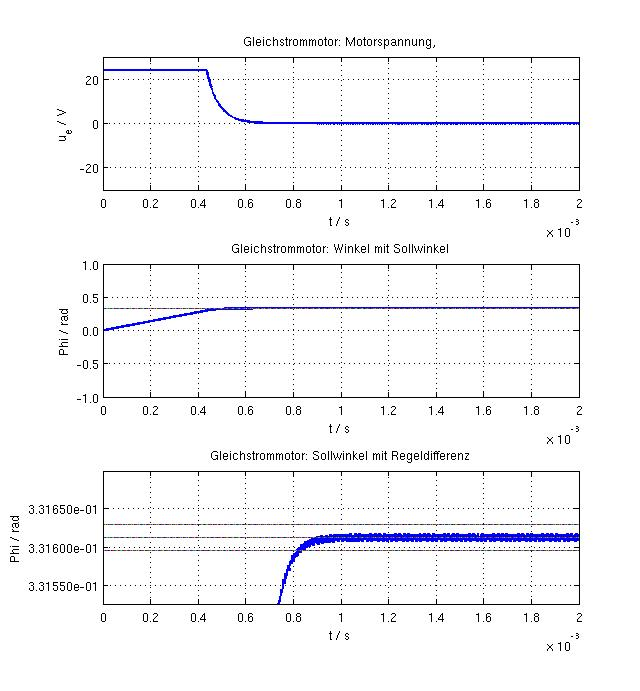
\includegraphics[width=0.6\textwidth]{Sensor_10_1_100_linear1.jpg}
	\caption{Erster linearer Sensor}
	\label{fig:linear1}
\end{figure}

\subsubsection{Linearer Sensor 2}
\label{chap:sensorregelung2}
Abb. \ref{fig:linear2} zeigt das Regelergebnis des zweiten linearen Sensors.
Es ist gut zu erkennen, dass eine Regeldifferenz übrig bleibt.
Diese lässt sich auch nicht durch verändern der Regelparameter reduzieren.
\begin{figure}[!h]
	\centering
	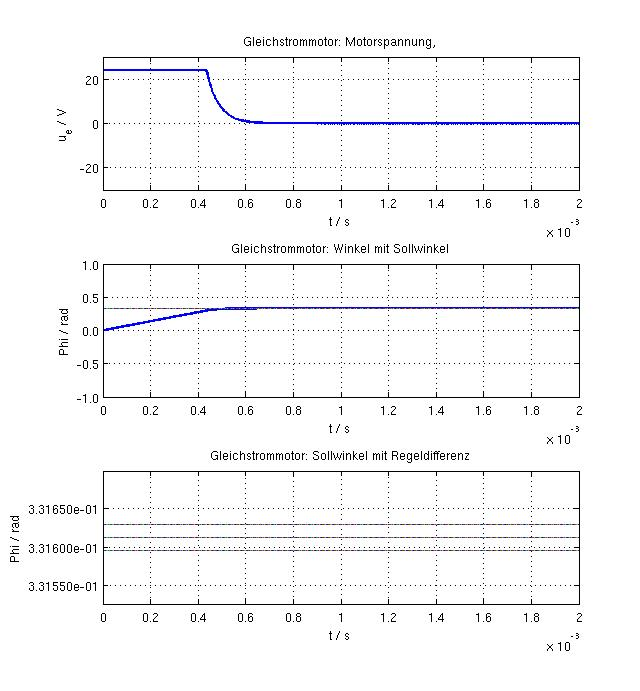
\includegraphics[width=0.6\textwidth]{Sensor_10_1_100_linear2.jpg}
	\caption{Zweier linearer Sensor}
	\label{fig:linear2}
\end{figure}

\subsubsection{Nichtlinearer Sensor}
\label{chap:sensorregelung3}
Abb. \ref{fig:nonlinear} zeigt das Regelergebnis des nicht linearen Sensors.
Auch hier ist eine restliche Regeldifferenz zu erkennen, die sich wiederum nicht durch anpassen der Regelparemeter begleichen lässt.
\begin{figure}[!h]
	\centering
	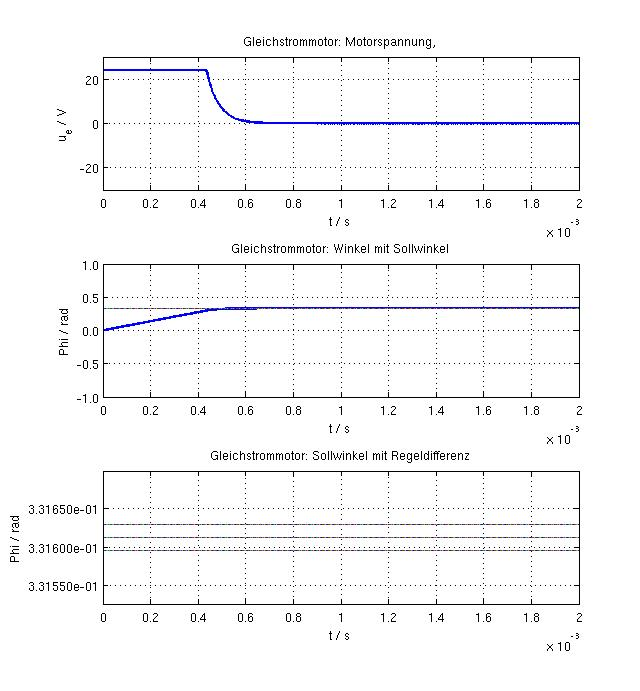
\includegraphics[width=0.6\textwidth]{Sensor_10_1_100_nonlinear00001.jpg}
	\caption{Linearer Sensor}
	\label{fig:nonlinear}
\end{figure}